
%%%%%%%%%%%%%%%%%%%%%%%%%%%%%%% Header %%%%%%%%%%%%%%%%%%%%%%%%%%%%%%%%%%%%%%%%%%%%
\begin{minipage}[l]{0.42\textwidth}
    
\includegraphics[width=1\textwidth]{img/logo-UNAMBA.png}
\end{minipage}
\hfill
\begin{minipage}[c]{0.5\textwidth}
    \begin{flushright}
	\large{\textbf{Unidad \#2}}\\
	\large{Lectures on Física I}\\
	\large{24 de julio del 2025. Haquira, Apurimac}\\
        % \large{\textbf{Student:} Huallpa Aimituma Josué David}
    \end{flushright}
\end{minipage}
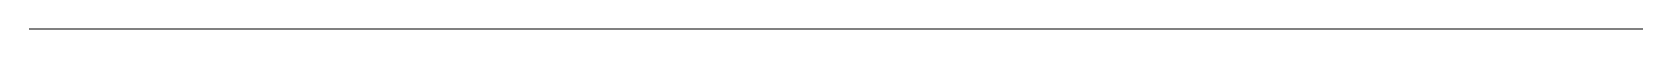
\begin{tikzpicture}
    \draw[gray,thick] (-6.5,0)--(14,0);
\end{tikzpicture}


 %%%%%%%%%%%%%%%%%%%%%%%% INICIO DEL CONTENIDO EN DOS COLUMNAS %%%%%%%%%%%%%%%%%%%%%

 \begin{multicols}{2}
     \begin{center}
         \LARGE{\textbf{Capítulo III: Estática}}\\	
         \vspace{0.2cm}
         % \Large {Lecturers Esteban Chalbaud \& Daniel Galviz} \\
         % \large{Teaching Assistant: Mauricio Gamonal \& Irvin Martínez}\\
         % \large{PhysicsLatam.com}\\
         % \vspace{0.2cm}
         \large{Fecha de entrega: 07 agosto 2025, 5:59 pm (GMT-4)}\\
         % \vspace{0.2cm}
         \large{— Evaluación pacial 2 —}
     \end{center}
          %%%%%%%%%%%%%%%%%%%%%%%%%%%%excercise%%%%%%%%%%%%%%%%%%%%%%%%%%%%%%%%%%%%%%%%
     \begin{excercise}[][][$F_x=286 \ \mathrm{lbf}$, $F_y=409\ \mathrm{lbf}$]{ex:0}{
        Un poste de telefono se mantiene en posición vertical mediante un cable fijo en el poste a una altura de 10 m e igualmente fijo al suelo a 7m de la base del poste. Si la tensión en el cable es de 500 lbf, ¿Cales son los valores de las fuerzas horizontales y verticales ejercidas sobre el poste por el cable? 
         }
     \end{excercise} 

     %%%%%%%%%%%%%%%%%%%%%%%%%%%%excercise%%%%%%%%%%%%%%%%%%%%%%%%%%%%%%%%%%%%%%%%
     \begin{excercise}[][][$(a)\ R =22 \ \mathrm{lbf}, \ \theta=25^\circ$, $(b)\ R =9.43 \ \mathrm{lbf}, \ \theta=72.8^\circ$, $(c)\ R =37 \ \mathrm{lbf}, \ \theta=-38.2^\circ$]{ex:1}{
         Encontrar la magnitud y la dirección de la resultante del sistema de fuerzas representadas en la Fig.
         \begin{figure}[H]
             \centering
             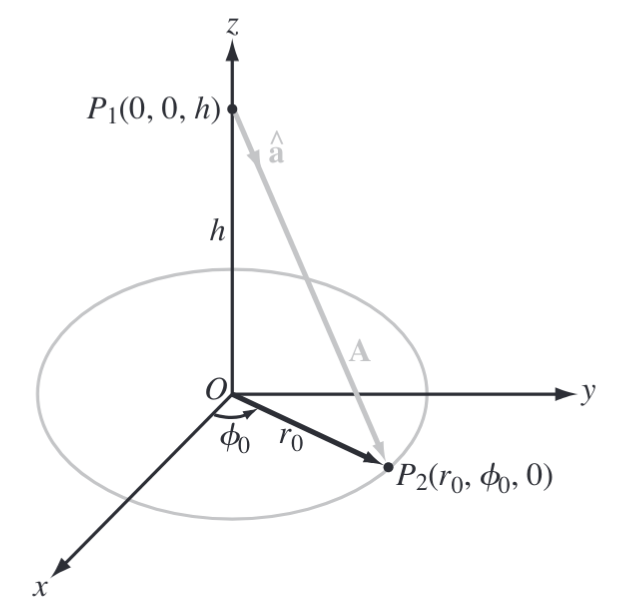
\includegraphics[width=0.75\linewidth]{img/01_physics-i/03_statics/1.png}
         \end{figure}
         }
     \end{excercise} 
     %%%%%%%%%%%%%%%%%%%%%%%%%%%%excercise%%%%%%%%%%%%%%%%%%%%%%%%%%%%%%%%%%%%%%%%
     \begin{excercise}[][][$R = 97.5\ \mathrm{N}$, $\theta=57.8$]{ex:2}{
         Cuatro fuerzas coplanares (30 N, 40 N, 20 N y 50 N) están todas actuando concurrentemente sobre un cuerpo. Los ángulos entre las fuerzas son, consecutivamente, $50^\circ$, $30^\circ$ y $60 ^\circ$. Calcular la magnitud de la fuerza resultante y el ángulo que hace con la fuerza de 30 N.
         }
     \end{excercise} 
     %%%%%%%%%%%%%%%%%%%%%%%%%%%%excercise%%%%%%%%%%%%%%%%%%%%%%%%%%%%%%%%%%%%%%%%
     \begin{excercise}[][][$(a) R= 525\ \mathrm{lbf}$, $\vec{e}_R=0.76\vec{\imath}$,  $(b) \tau=7900\ \mathrm{lbf\cdot ft}$]{ex:3}{
         Dadas las tres fuerzas siguientes: $F1 = 500\ \vec{\imath} $ lbf; $F_2 = -200\ \vec{\jmath} +  100\ \vec{k}$ lbf; $F_3 = -100 \ \vec{\imath} + 50\ \vec{\jmath} - 400 \vec{k} $ lbf. (a) Determinar la magnitud y dirección de la fuerza resultante. (b) Determinar el torque resultante de las fuerzas indicadas, con respecto al origen $\mathcal{O}$, si se aplican al punto $(4, -3, 15)$. Utilizar la fuerza resultante para determinar el torque resultante.
         }
     \end{excercise}    
     %%%%%%%%%%%%%%%%%%%%%%%%%%%excercise%%%%%%%%%%%%%%%%%%%%%%%%%%%%%%%%%%%%%%%%
     \begin{excercise}[][][$\vec{\tau} = 3150\vec{\imath}+7200\vec{\jmath}+600\vec{k}\ , \tau=7900\mathrm{lbf\cdot ft}$]{ex:4}{
          Calcular el torque, con respecto al origen $\mathcal{O}$, de cada una de las fuerzas dadas en el problema anterior , cuando cada una es aplicada en el punto $(4, -3, 15)$. Demostrar que el torque resultante es perpendicular a la fuerza resultante.
          }
      \end{excercise} 
      %%%%%%%%%%%%%%%%%%%%%%%%%%%%excercise%%%%%%%%%%%%%%%%%%%%%%%%%%%%%%%%%%%%%%%%
      \begin{excercise}[][][$(a)\tau=13000\ \mathrm{lbf\cdot ft}$, $(b)\tau_{min}=347\ \mathrm{lbf\cdot ft}$]{ex:5}{
          (a) Encontrar el torque resultante con respecto al punto de las fuerzas enumeradas en el problema anterior cuando se aplican en diferentes puntos: $F_1$ en $(3, 8, 10)$; $F_2$ en $(-2, 0, 4)$; $F_3$ en $(4, -25, 10)$. (b) Encontrar $\vec{R}\cdot\vec{\tau}$ e indicar la reducción mínima del sistema.
          }
      \end{excercise}
     %%%%%%%%%%%%%%%%%%%%%%%%%%%%excercise%%%%%%%%%%%%%%%%%%%%%%%%%%%%%%%%%%%%%%%%
      \begin{excercise}[][][$\tau= 24\sqrt{5}\ \mathrm{Nm}$, $y=0.5x+5$]{ex:6}{
         Calcular el torque de la fuerza en la figura con respecto al origen. Determinar la ecuación de la linea de acción de la fuerza. 
         \begin{figure}[H]
             \centering
             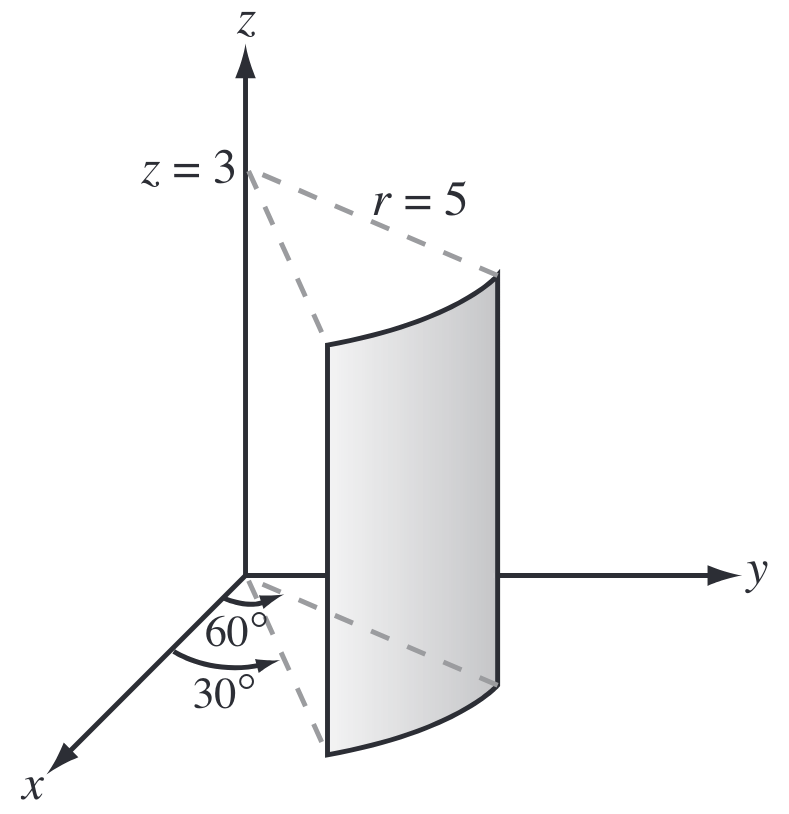
\includegraphics[width=0.53\linewidth]{img/01_physics-i/03_statics/2.png}
         \end{figure}
         }
     \end{excercise} 
     %%%%%%%%%%%%%%%%%%%%%%%%%%%%excercise%%%%%%%%%%%%%%%%%%%%%%%%%%%%%%%%%%%%%%%%
     \begin{excercise}[][][$(a)R=137.2\ \mathrm{N}$, $ \tau=0$, $(b)\ R=187.2\ \mathrm{N}$, $\tau=120\ \mathrm{Nm}$]{ex:7}{
         De la figura mostrada, determinar la fuerza y el torque resultantes con respecto a $\mathcal{O}$ de tres fuerzas, 50 N, 80 N, y 100 N, mutuamente perpendiculares entre sí. (a) Si son concurrentes. (b) Si la linea de acción de la fuerza de 100 N se encuentra a 1.2 m del punto de concurrencia de las otras dos.
         \begin{figure}[H]
             \centering
             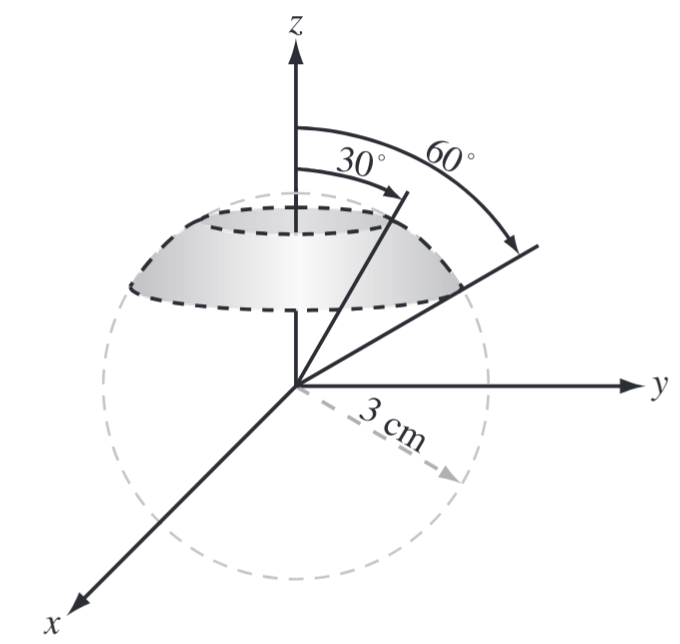
\includegraphics[width=0.9\linewidth]{img/01_physics-i/03_statics/3.png}
         \end{figure}
         }
     \end{excercise}
     %%%%%%%%%%%%%%%%%%%%%%%%%%%%excercise%%%%%%%%%%%%%%%%%%%%%%%%%%%%%%%%%%%%%%%%
     \begin{excercise}[][][$(a)\ R=3.975 \ \mathrm{N}$, $(b)\ \tau_{A}=1.4 \ \mathrm{Nm}$, $(c)\ \tau_{B}=5.33 \ \mathrm{Nm}$, $(d)\ \tau_{O}=1.5 \ \mathrm{Nm}$]{ex:8}{
         Sobre un rectángulo rígido ABCD de las siguientes dimensiones AB = CD 0,4 m y BC = DA = 0,6 m, actúan cinco fuerzas: en A, una fuerza de 6N en la dirección AB, una fuerza de 4N a lo largo de AC, y una fuerza de 3N a lo largo de AD; en C, una fuerza de 5N actuando a lo largo de la dirección CD y una fuerza de 4N actuando a lo largo de la dirección CB. Determinar la fuerza resultante, e igualmente el torque con respecto a los puntos A, B, y el centro geométrico.        
         }
     \end{excercise}

     %%%%%%%%%%%%%%%%%%%%%%%%%%%%excercise%%%%%%%%%%%%%%%%%%%%%%%%%%%%%%%%%%%%%%%%
     \begin{excercise}[][][$R=32.5\ \mathrm{N}$, $F_2=19.5\ \mathrm{N}$]{ex:9}{
         Dos fuerzas paralelas, y del mismo sentido, están separadas por una distancia de 0,2 m. Si una de las fuerzas es de 13N y la línea de acción de la resultante está a 0,08 m de la otra. encontrar (a) la magnitud de la resultante y (b) la magnitud de la otra fuerza.       
         }
     \end{excercise}
     %%%%%%%%%%%%%%%%%%%%%%%%%%%%excercise%%%%%%%%%%%%%%%%%%%%%%%%%%%%%%%%%%%%%%%%
     \begin{excercise}[][][$d=2m$]{ex:10}{
         Dos fuerzas paralelas, del mismo sentido, tienen magnitudes de 20N y 30N. La distancia de la línea de acción de la resultante a la fuerza mayor es de 0,8 m. Encontrar la distancia entre las fuerzas.   
         }
     \end{excercise}
     %%%%%%%%%%%%%%%%%%%%%%%%%%%%excercise%%%%%%%%%%%%%%%%%%%%%%%%%%%%%%%%%%%%%%%%
     \begin{excercise}[][][$R=22.2\ \mathrm{lbf}$, $y=-2.081x-3.65$]{ex:11}{
         Encontrar la magnitud y la posición de la resultante del sistema de fuerzas representadas en la fig. Las coordenadas de los puntos A, B y C se dan en pies.
         \begin{figure}[H]
             \centering
             \includegraphics[width=0.9\linewidth]{img/01_physics-i/03_statics/5.png}
         \end{figure}
         }
     \end{excercise}
     %%%%%%%%%%%%%%%%%%%%%%%%%%%%excercise%%%%%%%%%%%%%%%%%%%%%%%%%%%%%%%%%%%%%%%%
     \begin{excercise}[][][$R=25.7\ \mathrm{lbf}$, $y=$]{ex:12}{
         Encontrar la magnitud y la posición de la resultante de las fuerzas representadas en la Fig.  Cada cuadrado tiene 1 pie de lado.
         \begin{figure}[H]
             \centering
             \includegraphics[width=0.8\linewidth]{img/01_physics-i/03_statics/4.png}
         \end{figure}
         }
     \end{excercise}
     %%%%%%%%%%%%%%%%%%%%%%%%%%%%excercise%%%%%%%%%%%%%%%%%%%%%%%%%%%%%%%%%%%%%%%%
    \begin{excercise}[][][]{ex:13}{
            Demostrar que si $\vec{R} = \sum \vec{F}_i$ es la resultante de un sistema de fuerzas concurrentes y $\vec{\tau}_0$ es su torque con respecto al punto $\mathcal{O}$, el torque con respecto a A es $\vec{\tau}_A = \vec{\tau}_0 + \vec{r}_A \times \vec{R}$. 
         }
     \end{excercise}

     %%%%%%%%%%%%%%%%%%%%%%%%%%%%excercise%%%%%%%%%%%%%%%%%%%%%%%%%%%%%%%%%%%%%%%%
     \begin{excercise}[][][$R=6600\ \mathrm{dinas}$, $x_c=77.3 \ \mathrm{cm}$]{ex:14}{
        Una varilla tiene 2 m de largo y pesa 5 gmf (4900 dinas). Sobre ella actúan fuerzas de 3000, 2000, 1500 dinas que actúan hacia abajo a 0, 50 y 200 cm de un extremo, y fuerzas de 5000 y 13.000 dinas que actúan hacia arriba a 20 y 100 cm del mismo extremo.Determinar la magnitud y la línea de acción de la resultante.
         }
     \end{excercise}

     %%%%%%%%%%%%%%%%%%%%%%%%%%%%excercise%%%%%%%%%%%%%%%%%%%%%%%%%%%%%%%%%%%%%%%%
     \begin{excercise}[][][$R=-30\ \mathrm{Kgf}$, $x_c=56.7 \ \mathrm{cm}$, $R_A=8.8 \ \mathrm{Kgf}$, $R_B=21.2\ \mathrm{Kgf}$]{ex:15}{
         Encontrar la magnitud y posición de la resultante del sistema de fuerzas representado en la Fig. Cada segmento de la viga AB mide 1 dm. Encontrar también las fuerzas necesarias en A y B para balancear las otras fuerzas. 
         \begin{figure}[H]
             \centering
             \includegraphics[width=0.7\linewidth]{img/01_physics-i/03_statics/7.png}
         \end{figure}
         }
     \end{excercise}

     %%%%%%%%%%%%%%%%%%%%%%%%%%%%excercise%%%%%%%%%%%%%%%%%%%%%%%%%%%%%%%%%%%%%%%%
     \begin{excercise}[][][$R_A=1143 \ \mathrm{N}$, $R_B=1797\ \mathrm{N}$]{ex:16}{
         La viga AB es uniforme y tiene una masa de 100 kg. Descansa en sus extremos A y B y soporta las masas como se indica en la Fig. Calcular la reacción en los soportes.         
         \begin{figure}[H]
             \centering
             \includegraphics[width=0.7\linewidth]{img/01_physics-i/03_statics/8.png}
         \end{figure}
         }
     \end{excercise}
    %%%%%%%%%%%%%%%%%%%%%%%%%%%%excercise%%%%%%%%%%%%%%%%%%%%%%%%%%%%%%%%%%%%%%%%
     \begin{excercise}[][][$(a)\ T_1=T_2=26.1 \ \mathrm{lbf}$, $(b) T_1=56.4\ \mathrm{lbf}, T_2=40\ \mathrm{lbf}$, $(c)\ T_1=T_2=40 \ \mathrm{lbf}$, $(d) T_1=40\ \mathrm{lbf}, T_2=69.2\ \mathrm{lbf}$]{ex:17}{
         Determinar las tensiones sobre las cuerdas AC y BC si M pesa 40 lbf.   
         \begin{figure}[H]
             \centering
             \includegraphics[width=0.8\linewidth]{img/01_physics-i/03_statics/9.png}
             \includegraphics[width=0.8\linewidth]{img/01_physics-i/03_statics/10.png}
         \end{figure}
         }
     \end{excercise}

    %%%%%%%%%%%%%%%%%%%%%%%%%%%%excercise%%%%%%%%%%%%%%%%%%%%%%%%%%%%%%%%%%%%%%%%
     \begin{excercise}[img/01_physics-i/03_statics/11.png][\linewidth][$F=30 \ \mathrm{Kgf}$, $T=50\ \mathrm{Kgf}$]{ex:18}{
        El cuerpo representado en la figura pesa 40 kgf. Se mantiene en equilibrio por medio de una cuerda AB y bajo la acción de la fuerza horizontal F. Suponiendo que AB=150 cm y que la distancia entre la pared y el cuerpo es de 90 cm, calcular el valor de la fuerza F y la tensión en la cuerda
         } 
     \end{excercise}
    %%%%%%%%%%%%%%%%%%%%%%%%%%%%excercise%%%%%%%%%%%%%%%%%%%%%%%%%%%%%%%%%%%%%%%%
     \begin{excercise}[][][$\theta=53^\circ $, $T=500\ \mathrm{lbf}$]{ex:19}{
        Para la Fig. Calcular el ángulo y la tensión en la cuerda AB si $M_1=300$ lbf y $M_2=400$ lbf.     
         \begin{figure}[H]
             \centering
             \includegraphics[width=0.4\linewidth]{img/01_physics-i/03_statics/12.png}
         \end{figure}
    } 
     \end{excercise}
    
    %%%%%%%%%%%%%%%%%%%%%%%%%%%%excercise%%%%%%%%%%%%%%%%%%%%%%%%%%%%%%%%%%%%%%%%
     \begin{excercise}[][][$(a)=60\ \mathrm{lbf}$, $(b)=69 \ \mathrm{lbf}$]{ex:20}{
        Un muchacho que pesa 120 lbf sostiene una barra de levantamiento de pesas. ¿Qué fuerza ejerce cada uno de sus brazos sobre la barra cuando (a) sus brazos están en posición paralela y (b) cuando cada brazo hace un ángulo de $30^\circ$ con la vertical? Representar la fuerza en función del ángulo. ¿Qué conclusión obtiene Ud. de la gráfica?
         }
     \end{excercise}
    %%%%%%%%%%%%%%%%%%%%%%%%%%%%excercise%%%%%%%%%%%%%%%%%%%%%%%%%%%%%%%%%%%%%%%%
    \begin{excercise}[][][$P=4\ \mathrm{Kgf}$]{ex:21}{
       Una cuerda ABCD cuelga de los puntos fijos A y D. En B hay un peso de 12 kgf y en C un peso desconocido. Si el ángulo que hace AB con la horizontal es de $60^\circ$, BC es horizontal y CD hace un ángulo de $30^\circ$ con la horizontal, calcular el valor que P debe tener a fin de que el sistema se encuentre en equilibrio.         
        }
     \end{excercise}
    %%%%%%%%%%%%%%%%%%%%%%%%%%%%excercise%%%%%%%%%%%%%%%%%%%%%%%%%%%%%%%%%%%%%%%%
     \begin{excercise}[][][$T_3=73.3\ \mathrm{Kgf}$, $P=156.3 \ \mathrm{Kgf}$]{ex:22}{
       Tres cuerdas, situadas en un plano vertical, están fijas a puntos diferentes sobre el techo. Los otros extremos están unidos en el nudo A y del cual cuelga un peso P. Los ángulos formados por las cuerdas con la horizontal son, $35^\circ$, $100^\circ$ y $160^\circ$, respectivamente. Las tensiones en las primeras dos cuerdas son de 100 kgf y 75 kgf. Calcular la tensión en la tercera cuerda y el peso P.       
        }
     \end{excercise}
    %%%%%%%%%%%%%%%%%%%%%%%%%%%%excercise%%%%%%%%%%%%%%%%%%%%%%%%%%%%%%%%%%%%%%%%
     \begin{excercise}[][][$R_1=36.7\ \mathrm{Kgf}$, $R_2=25.9 \ \mathrm{Kgf}$]{ex:23}{
       Una esfera cuyo peso es de 50 kgf descansa sobre dos planos lisos, inclina- dos respectivamente con respecto a la horizontal, ángulos de $30^\circ$ y $45^\circ$. Calcular las reacciones de los dos planos sobre la esfera.       
        }
     \end{excercise} 
    %%%%%%%%%%%%%%%%%%%%%%%%%%%%excercise%%%%%%%%%%%%%%%%%%%%%%%%%%%%%%%%%%%%%%%%
     \begin{excercise}[img/01_physics-i/03_statics/13.png][0.9\linewidth][$R_1=86.7 \ \mathrm{lbf} $, $R_2=100\ \mathrm{lbf}$]{ex:24}{
        Una esfera (Fig.) que pesa 50 lbf descansa sobre una pared lisa, manteniéndose en esa posición mediante un plano liso que hace un ángulo de $60^\circ$ con la horizontal. Calcular la reacción de la pared y el plano sobre la esfera.   
        } 
     \end{excercise}    
    %%%%%%%%%%%%%%%%%%%%%%%%%%%%excercise%%%%%%%%%%%%%%%%%%%%%%%%%%%%%%%%%%%%%%%%
     \begin{excercise}[img/01_physics-i/03_statics/14.png][0.7\linewidth][$T=125.2 \ \mathrm{N} $, $R=75.4\ \mathrm{N}$]{ex:25}{
        Una esfera de peso $W=100$ N se sostiene mediante una cuerda AB (Fig.) y presiona una pared vertical lisa AC. Si $\alpha=37^\circ$ es el ángulo entre la cuerda y la pared, determinar la tensión en la cuerda y la reacción de la pared sobre la esfera.  
        } 
     \end{excercise}

    %%%%%%%%%%%%%%%%%%%%%%%%%%%%excercise%%%%%%%%%%%%%%%%%%%%%%%%%%%%%%%%%%%%%%%%
     \begin{excercise}[][][$(a)\ T=56.7\ \mathrm{Kgf} $, $R=40\ \mathrm{Kgf}$, $(b)\ T=69.2\ \mathrm{Kgf} $, $R=40\ \mathrm{Kgf}$]{ex:26}{
        Calcular las fuerzas (Fig.) que la viga AB y el cable AC ejercen en A, suponiendo que M pesa 40 kgf y que el peso del cable y la viga son despreciables.     
         \begin{figure}[H]
             \centering
             \includegraphics[width=0.8\linewidth]{img/01_physics-i/03_statics/15.png}
         \end{figure}
         } 
     \end{excercise}

    %%%%%%%%%%%%%%%%%%%%%%%%%%%%excercise%%%%%%%%%%%%%%%%%%%%%%%%%%%%%%%%%%%%%%%%
     \begin{excercise}[][][$x=3.17\ \mathrm{m} $, $R=40\ \mathrm{Kgf}$]{ex:27}{
        La viga uniforme AB de la Fig. tiene 4 m de largo y pesa 100 kgf. La viga puede rotar alrededor del punto fijo C. La viga reposa en el punto A. Un hombre que pesa 75 kgf camina a lo largo de la viga, partiendo de A. Calcular la máxima distancia que el hombre puede caminar a partir de A manteniendo el equilibrio. Representar la reacción en A como una función de la distancia x.   
         \begin{figure}[H]
             \centering
             \includegraphics[width=0.8\linewidth]{img/01_physics-i/03_statics/16.png}
         \end{figure}
         } 
     \end{excercise}     %%%%%%%%%%%%%%%%%%%%%%%%%%%%excercise%%%%%%%%%%%%%%%%%%%%%%%%%%%%%%%%%%%%%%%%
     \begin{excercise}[][][$W=54.6\ \mathrm{N}$]{ex:32}{
       En el sistema adjunto hallar el peso  W que produce el equilibrio 
         \begin{figure}[H]
             \centering
             \includegraphics[width=0.5\linewidth]{img/01_physics-i/03_statics/24.png}
         \end{figure}
         } 
     \end{excercise}
    %%%%%%%%%%%%%%%%%%%%%%%%%%%%excercise%%%%%%%%%%%%%%%%%%%%%%%%%%%%%%%%%%%%%%%%
     \begin{excercise}[][][$R=4170\ \mathrm{N} $, $x=196\ \mathrm{cm}$]{ex:28}{
        Sobre la viga AB actúan las fuerzas que se indican en la Fig. Determinar la magnitud y la posición de la resultante.     
         \begin{figure}[H]
             \centering
             \includegraphics[width=0.8\linewidth]{img/01_physics-i/03_statics/18.png}
         \end{figure}
         } 
     \end{excercise}
    
    %%%%%%%%%%%%%%%%%%%%%%%%%%%%excercise%%%%%%%%%%%%%%%%%%%%%%%%%%%%%%%%%%%%%%%%
     \begin{excercise}[][][$R_A=6690\ \mathrm{Kgf}$, $R_B=7010 \ \mathrm{Kgf}$]{ex:29}{
       Un puente de 100 m de largo y 10.000 kgf de peso se mantiene en posición horizontal mediante dos columnas situadas en sus extremos. ¿Cuáles son las reacciones sobre las columnas cuando hay tres carros sobre el puente a 30 m, 60 m y 80 m de uno de sus extremos, cuyos pesos son, respectivamente,1500 kgf, 1000 kgf y 1200 kgf?     
        }
     \end{excercise} 
    
    %%%%%%%%%%%%%%%%%%%%%%%%%%%%excercise%%%%%%%%%%%%%%%%%%%%%%%%%%%%%%%%%%%%%%%%
    \begin{excercise}[][][$P=587\ \mathrm{Kgf} $, $R=81.5\ \mathrm{Kgf}$]{ex:30}{
        Calcular el peso P necesario para mantener el equilibrio en el sistema mostrado en la Fig. En la cual A pesa 100 kgf y Q 10 kgf. El plano y las poleas son lisas. La cuerda AC es horizontal y la cuerda AB es paralela al plano. Calcular también la reacción del plano sobre el peso A.     
         \begin{figure}[H]
             \centering
             \includegraphics[width=0.7\linewidth]{img/01_physics-i/03_statics/19.png}
         \end{figure}
         } 
     \end{excercise}    %%%%%%%%%%%%%%%%%%%%%%%%%%%%excercise%%%%%%%%%%%%%%%%%%%%%%%%%%%%%%%%%%%%%%%%
    \begin{excercise}[][][$F_A=630.9\ \mathrm{Kgf} $, $R=509.1\ \mathrm{Kgf}$]{ex:31}{
        La barra de la fig, reposa en equilibrio sobre los puntos A y B, bajo la acción de las fuerzas que se indican. Encontrar las fuerzas ejercidas sobre la barra en los puntos A y B. La barra pesa 40 Kgf y su longitud es de 8m.
         \begin{figure}[H]
             \centering
             \includegraphics[width=0.8\linewidth]{img/01_physics-i/03_statics/22.png}
         \end{figure}
         } 
     \end{excercise}    %%%%%%%%%%%%%%%%%%%%%%%%%%%%excercise%%%%%%%%%%%%%%%%%%%%%%%%%%%%%%%%%%%%%%%%
    \begin{excercise}[][][$F_1=F_3=11.5\ \mathrm{lbf} $, $F_2=40\ \mathrm{lgf}$]{ex:32}{
        Una escalera AB de peso 40lbf descansa sobre una pared vertical, haciendo un ángulo de $60^\circ$ con el suelo. Encontrar las fuerzas sobre la escalera en A y B. La escalera tiene rodillos en A, de modo que la friccion es despreciable.   
        \begin{figure}[H]
             \centering
             \includegraphics[width=0.5\linewidth]{img/01_physics-i/03_statics/23.png}
         \end{figure}     
        } 
     \end{excercise}

\end{multicols}
